\documentclass{article}

\usepackage{amsmath,amssymb}
\usepackage{tikz}
\usetikzlibrary{er,positioning}
\usepackage{pgfplots}
\usepackage{xcolor}
\usepackage[left=2.1cm,right=3.1cm,bottom=3cm,footskip=0.75cm,headsep=0.5cm]{geometry}
\usepackage{enumerate}
\usepackage{enumitem}
\usepackage{marvosym}
\usepackage{tabularx}

\usepackage{listings}
\definecolor{lightlightgray}{rgb}{0.95,0.95,0.95}
\definecolor{lila}{rgb}{0.8,0,0.8}
\definecolor{mygray}{rgb}{0.5,0.5,0.5}
\definecolor{mygreen}{rgb}{0,0.8,0.26}
\lstdefinestyle{sql} {language=sql}
\lstset{language=sql,
	basicstyle=\ttfamily,
	keywordstyle=\color{lila},
	commentstyle=\color{lightgray},
	stringstyle=\color{mygreen}\ttfamily,
	backgroundcolor=\color{white},
	showstringspaces=false,
	numbers=left,
	numbersep=10pt,
	numberstyle=\color{mygray}\ttfamily,
	identifierstyle=\color{blue},
	xleftmargin=.1\textwidth, 
	%xrightmargin=.1\textwidth,
	escapechar=§,
}

\usepackage[utf8]{inputenc}

\renewcommand*{\arraystretch}{1.4}

\newcolumntype{L}[1]{>{\raggedright\arraybackslash}p{#1}}
\newcolumntype{R}[1]{>{\raggedleft\arraybackslash}p{#1}}
\newcolumntype{C}[1]{>{\centering\let\newline\\\arraybackslash\hspace{0pt}}m{#1}}

\newcommand{\E}{\mathbb{E}}
\DeclareMathOperator{\rk}{rk}
\DeclareMathOperator{\Var}{Var}
\DeclareMathOperator{\Cov}{Cov}
\DeclareMathOperator{\Hul}{Hul}

\def\ojoin{\setbox0=\hbox{$\bowtie$}%
	\rule[-.02ex]{.25em}{.4pt}\llap{\rule[\ht0]{.25em}{.4pt}}}
\def\leftouterjoin{\mathbin{\ojoin\mkern-5.8mu\bowtie}}
\def\rightouterjoin{\mathbin{\bowtie\mkern-5.8mu\ojoin}}
\def\fullouterjoin{\mathbin{\ojoin\mkern-5.8mu\bowtie\mkern-5.8mu\ojoin}}

\title{\textbf{Datenbanken, Übung 7}}
\author{\textsc{Henry Haustein}}
\date{}

\begin{document}
	\maketitle
	
	\section*{Aufgabe 1}
	\begin{itemize}
		\item A - Atomarität (alles oder nichts, es gibt keine halben Transaktionen): Alle Operationen einer Transaktion müssen atomar, das heißt ganz oder gar nicht ausgeführt werden.
		\item C - Konsistenz (eine Transaktion muss einen konsistenten Zustand hinterlassen): Die von einer Transaktion durchgeführten Operationen müssen das Datenbanksystem von einem konsistenten Zustand wieder in einen konsistenten Zustand überführen.
		\item I - Isolation (jede Transaktion läuft so, als wäre Sie allein auf der Datenbank): Mehrere nebenläufige Transaktionen müssen voneinander isoliert werden, das heißt die Transaktionen dürfen sich nicht gegenseitig beeinflussen.
		\item D - Dauerhaftigkeit (nach einem Commit müssen die Daten dauerhaft gespeichert werden): Die von einer erfolgreich abgeschlossenen Transaktion (commit) durchgeführten Änderungen dürfen  - auch im Fall von Systemfehlern - nicht verloren gehen, das heißt die Änderungen müssen dauerhaft erhalten bleiben.
	\end{itemize}

	\section*{Aufgabe 2}
	\begin{enumerate}[label=(\alph*)]
		\item Verzahnung von $T_1$ und $T_2$:
		\begin{center}
			\begin{tabular}{c|c}
				$T_1$ & $T_2$ \\
				\hline
				BOT$_1$ & \\
				Read$_1$(B) & \\
				Write$_1$(A) & \\
				Read$_1$(B) & \\
				& BOT$_2$ \\
				& Read$_2$(B) \\
				& Read$_2$(A) \\
				Write$_1$(B) & \\
				Commit$_1$ & \\
				& Write$_2$(B) \\
				& Commit$_2$
			\end{tabular}
		\end{center}
		\item Verzahnung von $T_2$ und $T_3$
		\begin{center}
			\begin{tabular}{c|c}
				$T_2$ & $T_3$ \\
				\hline
				& BOT$_3$ \\
				& Read$_3$(B) \\
				& Write$_3$(B) \\
				BOT$_2$ & \\
				Read$_2$(B) & \\
				Read$_2$(A) & \\
				Write$_2$(B) & \\
				Commit$_2$ & \\
				& Abort$_3$
			\end{tabular}
		\end{center}
		\item Verzahnung von $T_1$ und $T_2$
		\begin{center}
			\begin{tabular}{c|c}
				$T_1$ & $T_2$ \\
				\hline
				BOT$_1$ & \\
				Read$_1$(B) & \\
				& BOT$_2$ \\
				& Read$_2$(B) \\
				& Read$_2$(A) \\
				& Write$_2$(B) \\
				& Commit$_2$ \\
				Write$_1$(A) & \\
				Read$_1$(B) & \\
				Write$_1$(B) & \\
				Commit$_1$ & 
			\end{tabular}
		\end{center}
	\end{enumerate}

	\section*{Aufgabe 3}
	\begin{enumerate}[label=(\alph*)]
		\item Es gibt in diesem Graphen sehr viele Konfliktoperationen, deswegen hier die Aufzählung einiger:
		\begin{itemize}
			\item zwischen Schritt 4 und 5: $w_2(B) < r_1(B)$
			\item zwischen Schritt 6 und 7: $w_1(A) < r_2(A)$
			\item zwischen Schritt 9 und 10: $w_2(A) < r_3(A)$
			\item zwischen Schritt 8 und 11: $w_2(C) < r_3(C)$
			\item zwischen Schritt 4 und 12: $w_2(B) < w_1(B)$
			\item zwischen Schritt 6 und 10: $w_1(A) < r_3(A)$
		\end{itemize}
		\item Man erkennt, dass in jedem Fall $T_2<T_1$, $T_1<T_2$, $T_2<T_3$ und $T_1<T_3$ gelten sollte. Daraus kann man den folgenden Serialisierbarkeitsgraphen erstellen:
		\begin{center}
			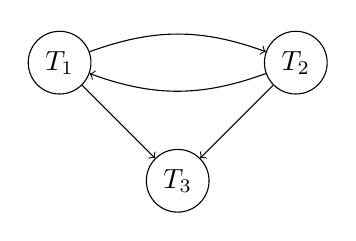
\begin{tikzpicture}
			\node[circle,draw=black, fill=white] (T1) at (0,0) {$T_1$};
			\node[circle,draw=black, fill=white] (T2) at (3,0) {$T_2$};
			\node[circle,draw=black, fill=white] (T3) at (1.5,-1.5) {$T_3$};
			
			\draw[->] (T1) to[bend left=20] (T2);
			\draw[->] (T2) to[bend left=20] (T1);
			\draw[->] (T1) -- (T3);
			\draw[->] (T2) -- (T3);
			\end{tikzpicture}
		\end{center}
		\item Serialisierbar wäre der Ablaufplan, wenn im Graphen kein Zyklus auftritt. Es tritt allerdings ein Zyklus auf, deswegen ist der Ablaufplan nicht serialisierbar.
	\end{enumerate}
	
	\section*{Aufgabe 4}
	\begin{enumerate}[label=(\alph*)]
		\item Die Historie ist seriell, damit auch serialisierbar, rücksetzbar, verhindert kaskadierendes Rücksetzen und ist strikt.
		\item Diese Historie ist offensichtlich nicht seriell und auch nicht serialisierbar, da wegen $w_1(x) < w_2(x)$ und $w_2(y) < w_1(y)$ gilt: $T_1 < T_2$ und $T_2 < T_1$. Beides kann nicht gleichzeitig gelten. Da in dieser Historie keine Reads stattfinden, ist die Historie auch rücksetzbar. Mit dem gleichen Argument verhindert sie auch kaskadierendes Rücksetzen, aber strikt ist die Historie nicht, da in der Historie Daten von $T_2$ verarbeitet werden, bevor der Commit von $T_1$ geschieht.
		\item Auch hier ist die Historie nicht seriell und wegen $w_1(x) < r_2(x)$, aber $w_2(y) < r_1(y)$ ist die Historie auch nicht serialisierbar. Wegen $w_2(y) < r_1(y)$, aber $c_1 < c_2$ folgt damit, dass die Historie nicht rücksetzbar, damit nicht kaskadierendes Rücksetzen vermeidet und auch nicht strikt.
		\item Die Historie ist nicht seriell, aber serialisierbar mit $T_1 < T_2$. Und da auch $c_1 < c_2$ ist die Historie rücksetzbar. Aber da $w_1(x) < r_2(x) < ... < c_1$ liest diese Historie auch nicht abgeschlossenen Transaktionen und verhindert damit nicht kaskadierendes Zurücksetzen. Damit ist die Historie auch nicht strikt.
	\end{enumerate}

	\section*{Aufgabe 5}
	\begin{enumerate}[label=(\alph*)]
		\item Die Serialisierbarkeit wird gewährleistet, die Rücksetzbarkeit nicht, z.B. bei folgender Historie nicht:
		\begin{align}
			w_1(x) \quad r_2(x) \quad w_2(y) \quad c_2\quad c_1 \notag
		\end{align}
		$T_1$ gibt hier nach $w_1(x)$ eine Sperre auf und damit kann sich $T_2$ vor $T_1$ drängeln. Damit ist auch nicht die Vermeidung vom kaskadierendem Rücksetzen und die Striktheit gewährleistet.
		\item Da alle Sperren bis zum Commit gehalten werden, ist kein Vordrängeln möglich und die Historien sind rücksetzbar, vermeiden kaskadierendes Rücksetzen und sind strikt.
	\end{enumerate}

	\section*{Aufgabe 6}
	Wartegraph aus den Sperren \textcolor{blue}{$T_1(X,c)$}, \textcolor{red}{$T_2(S,f)$}, \textcolor{green!80!black}{$T_3(X,b)$}, \textcolor{orange}{$T_4(S,a)$}, \textcolor{violet}{$T_5(X,d)$}
	\begin{center}
		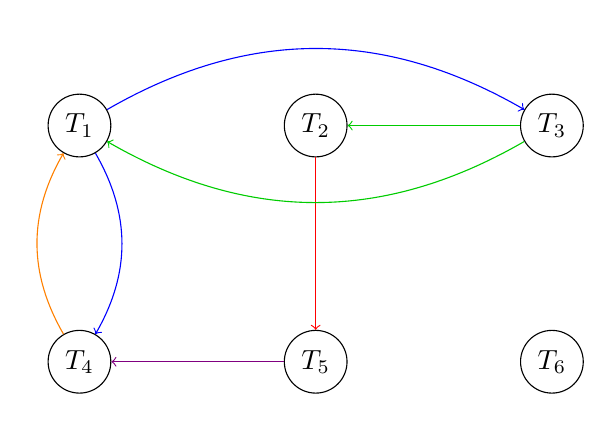
\begin{tikzpicture}
		\node[circle,draw=black, fill=white] (T1) at (0,0) {$T_1$};
		\node[circle,draw=black, fill=white] (T2) at (3,0) {$T_2$};
		\node[circle,draw=black, fill=white] (T3) at (6,0) {$T_3$};
		\node[circle,draw=black, fill=white] (T4) at (0,-3) {$T_4$};
		\node[circle,draw=black, fill=white] (T5) at (3,-3) {$T_5$};
		\node[circle,draw=black, fill=white] (T6) at (6,-3) {$T_6$};
		
		\draw[->,blue] (T1) to[bend left=30] (T3);
		\draw[->,blue] (T1) to[bend left=30] (T4);
		\draw[->,red] (T2) -- (T5);
		\draw[->,green!80!black] (T3) to[bend left=30] (T1);
		\draw[->,green!80!black] (T3) -- (T2);
		\draw[->,orange] (T4) to[bend left=30] (T1);
		\draw[->,violet] (T5) -- (T4);
		\end{tikzpicture}
	\end{center}
	
\end{document}